\documentclass[a4paper, 12pt]{article}
\usepackage{cmap}           % Пакет для поиска в полученной пдфке
\usepackage[utf8]{inputenc} % Ззамена кодировки файла на utf8
\usepackage[T2A]{fontenc}   % Подключение кодировки шрифтов
\usepackage[russian]{babel} % Использование русского языка 
\usepackage[left=2cm, right=2cm, top=1cm, bottom=2cm]{geometry} % Изменение размеров полей
\usepackage{indentfirst}    % Красная строка в начале текста
\usepackage{amsmath, amsfonts, amsthm, mathtools, amssymb, icomma, units, yfonts}
\usepackage{amsthm} % Пакет для нормального оформления теорем
\usepackage{algorithmicx, algorithm}
\usepackage{algpseudocode}
\usepackage{graphicx}
\usepackage{tikz}
\usepackage{esvect}
\usepackage{enumitem}
\usetikzlibrary{calc,matrix}

%Теоремы
%11.01.2016
\newtheorem*{standartbase}{Теорема о стандартном базисе}
\newtheorem*{fulllemma}{Лемма}
\newtheorem*{sl1}{Следствие 1}
\newtheorem*{sl2}{Следствие 2}
\newtheorem*{monotonousbase}{Теорема о монотонном базисе}
\newtheorem*{scheme}{Утверждение 1}
\newtheorem*{n2}{Утверждение 2}
\newtheorem*{usp-rais}{Теорема Успенского-Райса}
\newtheorem*{rec}{Свойство рекурсии}
\newtheorem*{point}{Теорема о неподвижной точке}
\newtheorem*{zhegalkin}{Теорема Жегалкина}
\newtheorem*{poste}{Теорема Поста}
\newtheorem*{algo1}{Первое свойство алгоритмов}



%18.01.2016
\newtheorem*{theorem}{Теорема}

\renewcommand{\qedsymbol}{\textbf{Q.E.D.}}
\newcommand{\definition}{\underline{Определение:} }
\newcommand{\definitions}{\underline{Определения:} }
\newcommand{\definitionone}{\underline{Определение 1:} }
\newcommand{\definitiontwo}{\underline{Определение 2:} }
\newcommand{\statement}{\underline{Утверждение:} }
\newcommand{\note}{\underline{Замечание:} }
\newcommand{\sign}{\underline{Обозначения:} }
\newcommand{\statements}{\underline{Утверждения:} }

\newcommand{\Z}{\mathbb{Z}}
\newcommand{\N}{\mathbb{N}}
\newcommand{\Q}{\mathbb{Q}}
\newcommand{\R}{\mathbb{R}}



\begin{document}
\title{Дискретная математика.\\ Коллоквиум.}
\author{Лекторий ПМИ ФКН 2015-2016\\ Определения 1 и 2: Вельдяйкин Николай и Бубнова Валерия \\ Определения 3 и 4, Вероятность и Машины Тьюринга: Гринберг Вадим \\ Дополнение 10: Вельдякин Николай}
\date{16-21 марта 2016}

\maketitle

\part*{Определения}

\section*{1. Функции, определение с помощью графика функции. Образы и прообразы множеств}
\textit{По простому:} Функция  $f$ -- когда каждому элементу $x$ из некоторого множества, области определения функции, поставлен в соответствие какой-то элемент $f(x)$ другого множества, области значений, причём только один. 
\\
\textit{Формально:} говорят, что на множестве $X$ имеется функция $f$ со значениями из $Y$, если некоторым элементам $x$ из множества $X$ по правилу $f$ поставлен в соответствие некоторые элементы $y$ из множества $Y$.

\par Говорят также, что функция $f\ \textit{отображает}$ множество $X$ в множество $Y$. Функцию обозначают также записью $y = f(x)$.

$Y$ -- область значения функции. $X$ -- область задания функции.

\par Используя понятие бинарного отношения, можно определить понятие функции как частный случай. А именно, отношение $F \subseteq A \times B$ называется функцией из $A$ в $B$, если каждый элемент множества $A$ находится в отношении $F$ не более чем с одним элементом множества $B$.
\par Альтернативно: если в $F$ нет двух пар с одинаковой первой компонентой и разными вторыми. 
\par Альтернативно:
\par Функцией $f:X \to Y$  называется множество $f$ упорядоченных пар $(x,\ y) \in X \times Y$, таких, что для любого элемента $x \in X$ существует единственный элемент $y \in Y$ такой, что:
\begin{itemize}
\item множество $\{y\}$, таких, что $(x,\ y) \in f$ для некоторых элементов $x \in X$, называется \textit{множеством значений функции}.
\item множество упорядоченных пар $f \subseteq X \times Y$ называется \textit{графиком функции}. Понятия графика и функции как множества упорядоченных пар совпадают. При обычном определении функции её графиком называется множество пар $(x,\ f(x))$.
\end{itemize}

\par Не требуется, чтобы всякий элемент $x \in A$ находился в отношении $F$ с каким-то элементом в $B$, важно только, чтобы он не находился в отношении $F$ с двумя разными элементами $B$. Так что для данного $x \in A$ может либо не быть никакого элемента в $B$, находящегося с $x$ в отношении $F$, либо быть ровно один такой элемент $y$. Во втором случае говорят, что $x$ входит в область определения функции $F$, а этот самый единственный элемент $y$, находящийся в отношении $F$ с $x$, называют значением функции $F$ на $x$ и обозначают $F(x)$. Элементы $F(x)$ для всех $x$ из области определения функции $F$ образуют множество значений функции $F$. Другими словами, множество значений функции $F$ -- это множество элементов в $B$, находящихся в отношении $F$ с некоторым элементом в $A$.

\par Если область определения функции совпадает с $A$, то пишут $f : A \to B$.Такие функции еще называют \textit{всюду определенными}, а иногда \textit{тотальными} в отличие от общего случая частичных функций.

\par Для функции $f$, аргументами и значениями которой являются действительные числа, можно нарисовать на плоскости её \textit{график} -- множество всех точек с координатами $(x,\ f(x))$. Иными словами: график функции $f(x)$ -- все точки с координатами $(x,\ y)$ такими, что $y = f(x)$.

\par Можно сказать, что функции $f: X \to Y$  и $g: X^{'} \to Y^{'}$  называются \textit{равными} при обычном их определении, если у них совпадают графики.

\par Элемент $y = f(x)$, который сопоставлен элементу $x$, называется \textit{образом элемента} (точки) $x$ (при отображении $f$).

\par Если взять целиком подмножество $A$ области задания функции $f$, то можно рассмотреть совокупность образов всех элементов множества  $A$, а именно подмножество области значений (функции $f$) вида
\begin{equation}
f(A) := \{f(x)\ |\ x \in A\} 
\end{equation}
которое называется образом множества $A$ при отображении $f$. 

\par Наоборот, взяв некоторое подмножество $B$ области значений функции $f$, можно рассмотреть совокупность тех элементов области задания функции $f$, чьи образы попадают в множество $B$, а именно -- множество вида
\begin{equation}
f^{-1}(B) := \{x\ |\ f(x) \in B\} 
\end{equation}
которое называется (полным) прообразом множества $B$ (при отображении $f$).
В том частном случае, когда множество $B$ состоит из одного элемента, скажем, $B = \{y\}$ , множество $f^{-1}(\{y\}) := \{f(x)\ |\ x \in y\}$ имеет более простое обозначение $f^{-1}(y)$.

\section*{2. Виды функций: инъекции, сюръекции, биекции}
Рассмотрим некоторое сопоставление элементов из множества $A$ в множество $B$. Будем называть его \textit{функцией}, если оно соответствует критерию \textit{функциональности}. Это значит, что каждому элементу $A$ соответсвтвует \textsc{не более} одного элемента из $B$ (строго: $(a,\ b) \in f, (a,\ c) \in f \implies b = c$). Далее будем считать, что это сопоставление является некоторой функцией $f: A \mapsto B$.

\textit{Инъекция} --- одному элементу из $B$ соответствует только один элемент из $A$. Строго говоря, $(a,\ c) \in f, (b,\ c)\in f \implies a = b$ или $a \neq b \implies f(a) \neq f(b)$. При этом $|A| \leq |B|$

\begin{center}
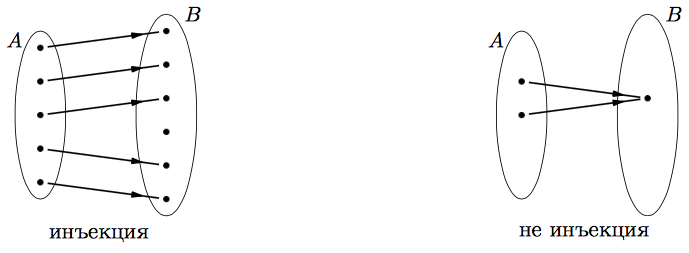
\includegraphics[height=3cm]{images/in.png}
\end{center}

\textit{Сюръекция} --- каждому элементу из $B$ что-то из $A$ да соответсвтует. Строго говоря, $\forall\ b \in B\ \exists\ a:\ f(a) = b$ и $|A| \geq |B|$

\begin{center}
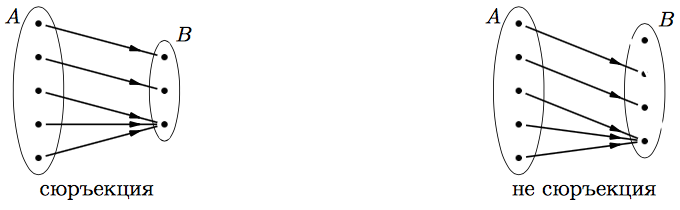
\includegraphics[height=3cm]{images/sur.png}
\end{center}

\textit{Биекция} --- и то, и другое: каждому элементу из $B$ соответствует элемент из $A$, притом только один. То есть это и $(a,\ c) \in f, (b,\ c)\in f \implies a = b$, и $\forall\ b \in B\ \exists\ a:\ f(a) = b$. При этом $|A| = |B|$.

\begin{center}
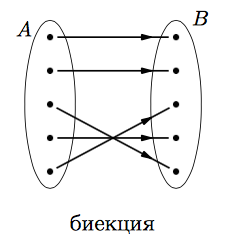
\includegraphics[height=3cm]{images/bi.png}
\end{center}

Заметим, что эти свойства определены только для всюду определенных функций (отображений), которыми являются не все функции.

\section*{3. Композиция функций, ее свойства.}
Пусть даны функции $f: A \to B$ и $g: B \to C$. Их композицией называется функция $g \circ f: A \to C$,
которая определена на тех $x$ из области определения $f$, для которых $f(x)$ принадлежит области определения $g$, и равна $g(f(x))$.

\begin{figure}[h]
\begin{center}
    \begin{minipage}[h]{0.6\linewidth}
        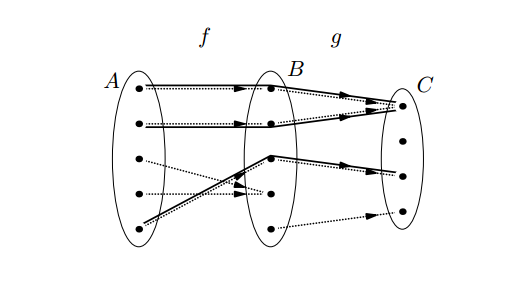
\includegraphics[height=5cm, width=\linewidth]{images/Comp.png}
        \caption{Композиция функций $f$ и $g$.}
    \end{minipage}
\end{center}
\end{figure}

Обратите внимание, что в записи $g \circ f$ мы сначала пишем ту функцию, которая применяется второй, -- просто потому, что такой же порядок в записи $g(f(x))$.

Композиция функций обладает свойством ассоциативности
$(f \circ g) \circ h = f \circ (g \circ h)$.
Здесь мы предполагаем, что множества, для которых определены функции, выбраны согласованно, то есть $h$ это функция из множества $A$ в множество $B$, $g$ это функция из множества $B$ в множество $C$, а $f$ это функция из множества $C$ в множество
$D$ (иначе композиции нельзя определить).

Ассоциативность проще понять, чем объяснить: обе части равенства задают функции $r_1$ и $r_2$ из множества $A$ в множество $D$. Равенство $y = r_1(x)$ равносильно тому,
что найдётся такое $z \in B$, что выполняются равенства $z = h(x)$, $y = (f \circ g)(z) = f(g(z))$.

Обозначим $u = g(z)$. Тогда $u = (g \circ h)(x)$ и $y = f(u)$, что по определению равносильно $y = r_2(x)$.
В обратную сторону рассуждение аналогичное.

\section*{4. Обратная функция, ее свойства.}
Тождественной функцией на множестве $A$ (или тождественным отображением множества $A$ в себя) называется функция $id_A$: $A \to A$, которая отображает всякий элемент $x \in A$ в себя: $id_A(x) = x$. При композиции тождественные функции ведут
себя, как единица при умножении: для любого отображения $f : A\to B$ выполнены равенства:

\[
    id_B \circ f = f \circ id_A = f.
\]
(Обратите внимание, что здесь две тождественные функции — одна на $A$, другая на $B$, иначе композицию нельзя определить.)

Если отображение $f : A \to B$ является биекцией (взаимно однозначным соответствием), то можно определить обратную функцию (или обратное отображение) $f^{-1}$:
если $f$ отображает $x$ в $y$, то обратная функция $f^{-1}$ отображает $y$ в $x$. Инъективность $f$ гарантирует, что это действительно функция, а сюръективность $f$ гарантирует,
что эта функция определена на всём $B$.
Заметим, что определение обратной функции симметрично: если $g$ обратна к $f$, то и $f$ обратна к $g$.

\statement{Для биекции $f : A \to B$ выполнены равенства

\[
    f^{-1} \circ f = id_A \text{и} f \circ f^{-1} = id_B
\]
}

\begin{proof}
Возьмём $x \in A$. Пусть $f(x) = y$. Тогда по определению обратной
функции $f^{-1}(y) = x$, а по определению композиции $(f^{-1} \circ f)(x) = f^{-1}(f(x)) = f^{-1}(y) = x$. Значит, $(f^{-1} \circ f) = id_A$.Возьмём $y \in B$. Пусть $f^{-1}(y) = x$. Тогда по определению обратной функции $f(x) = y$, а по определению композиции $(f \circ f^{-1})(y) = f(f^{-1}(y)) = f(x) = y$. Значит, $(f \circ f^{-1}) = id_B$.

\end{proof}

\section*{5. Основные определения элементарной теории вероятностей: исходы, события, вероятность события.}

Вероятностным пространством называется конечное множество $U$, его элементы называются возможными исходами. На вероятностном пространстве задана функция $Pr: U \to [0,\ 1]$, такая что $\sum\limits_{x \in U} Pr[x] = 1$. Функция $Pr$ называется вероятностным распределением, а число $Pr[x]$ называется вероятностью исхода $x \in U$. Событием называется произвольное подмножество $A \subseteq U$. Вероятностью события $A$ называется число $Pr[A] = \sum\limits_{x \in A} Pr[x]$.


\section*{6. Условная вероятность.}

Условной вероятностью события $A$ при условии $B$ называется число

\[
    Pr[A|B] = \frac{Pr[A \cap B]}{Pr[B]}
\]

Заметим, что условная вероятность имеет смысл, только если $Pr[B] > 0$. Иначе знаменатель обращается в ноль.

Определение условной вероятности можно переписать следующим образом:
\[
    Pr[A \cap B] = Pr[B] \cdot Pr[A|B]
\]

Другими словами, чтобы найти вероятность пересечения событий $A$ и $B$ достаточно найти вероятность события $B$ и условную вероятность события $A$ при условии события $B$.


\section*{7. Независимые события. Основные свойства независимых событий.}

Cобытие $A$ не зависит от события $B$, если

\[
    Pr[A] = Pr[A|B]
\]

Чтобы не возникало никаких тонкостей с нулевыми вероятностями полезно условиться, что вероятности событий $A$ и $B$ ненулевые.
Из определения условной вероятности мы сразу получаем эквивалентное определение независимости событий. Событие $A$ не зависит от события $B$, если 

\[
    Pr[A \cap B] = Pr[A] \cdot Pr[B]
\]

Из этой формы определения видно замечательное свойство независимости событий: она симметрична. То есть, событие $A$ не зависит от события $B$ тогда и только тогда, когда событие $B$ не зависит от события $A$.

Отметим также, что если события $A$ и $B$ независимы, и вероятность события $\overline{B}$ положительна, то события $A$ и $\overline{B}$ независимы.

\section*{8. Случайная величина.}

Случайная величина -- это числовая функция на вероятностном пространстве, то есть функция вида $f : U \to R$. То есть, по сути, случайная величина -- это обычная числовая функция, но теперь на её аргументах задано вероятностное распределение. Таким образом, например, мы можем говорить о вероятности того, что случайная
величина $f$ равна какому-то конкретному значению $a$: это есть просто вероятность события $\{u \in U\ |\ f(u) = a \}$. Случайные величины представляют собой числовые характеристики вероятностных экспериментов, и на самом деле, мы с ними уже неоднократно сталкивались, просто не говорили об этом. Например, если мы бросаем кубик, то исходом эксперимента является выпадение той или иной грани, а случайной величиной -- число написанное на грани (каждой грани соответствует своё число -- это функция).

\section*{9. Математическое ожидание случайной величины.}

Пусть вероятностное событие состоит из $k$ исходов, случайная величина $f : U \to R$ принимает на них значения $a_1, \ldots ,\ a_k$ соответственно и вероятности исходов равны $p_1, \ldots ,\ p_k$ соответственно. В частности, $\sum\limits_{i = 1}^k p_i = 1$. Предположим, что мы повторяем эксперимент по выбору случайного элемента из $U$ $n$ раз. Если $n$ достаточно большое, то случайная величина $f$ примет значение $a_1$ примерно $p_1n$ раз, значение $a_2$ -- примерно $p_2n$ раз, и так далее, значение $a_k$ -- примерно $p_kn$ раз. Подсчитаем теперь примерное среднее арифметическое значений случайной величины $f$ в этих экспериментах:

\[
    \frac{a_1p_1n + a_2p_2n + \ldots + a_kp_kn}{n} = \sum\limits_{i = 1}^k a_ip_i
\]

Математическим ожиданием случайной величины $f$, принимающей значения $a_1, \ldots ,\ a_k$ с вероятностями $p_1, \ldots ,\ p_k$ соответственно, называется величина 

\[
    E[f] = \sum\limits_{i = 1}^k a_ip_i
\]

\section*{10. Определение схемы в некотором функциональном базисе. Представление схем графами.}

\textit{Схема} --- это функция, заданная последовательностью присваиваний.

Иными словами, булевой схемой от переменных $x_1,\ \ldots\ ,\ x_n$ мы будем называть последовательность
булевых функций $g_1,\ \ldots\ ,\ g_s$, в которой всякая $g_i$ или равна одной из переменных, или
получается из предыдущих применением одной из логических операций отрицание,
конъюнкция и дизъюнкция.

Также в профессиональной среде схемы называют SLP (\textit{straight line programmes}). 

Рассмотрим такую функцию $f$, определенную для булевых значений (\textit{булеву функцию}): $f:\{0, 1\}^n \rightarrow \{0, 1\}$.

\textit{Базисом} $B$ булевой функции будем называть некий набор $B:\{f_1, f_2, \ldots , f_n\}$, где $f_1 \ldots f_n$ - булевы функции.

\textit{Булева схема} в базисе $B$  --- последовательность функций $x_1, x_2, x_3... x_n, x_{n+1} := S_1, x_L := S_{L-n}$, которая вычисляет $x_L(x_1, \ldots ,x_n)$. 

\[S_j = g(S_{i_1},  ... , s_{i_r}), g \in B, i_\mathalpha < j\]

\textit{Стандартный базис} есть базис, состоящий из операций отрицания, конъюнкции и дизъюнкции: $\{\lnot, \vee, \wedge\}$

Схемы можно предствавлять в виде графов:

\textsc{Пример 1}

Зададим булеву схему с помощью стандартного базиса.

$x_1, \ldots ,x_n, s_1 := \lnot x_1, s_2 = \lnot x_2, s_3 := x_1 \wedge s_2, s_4 := x_2 \wedge s_1; s_5 := s_3 \vee s_4$

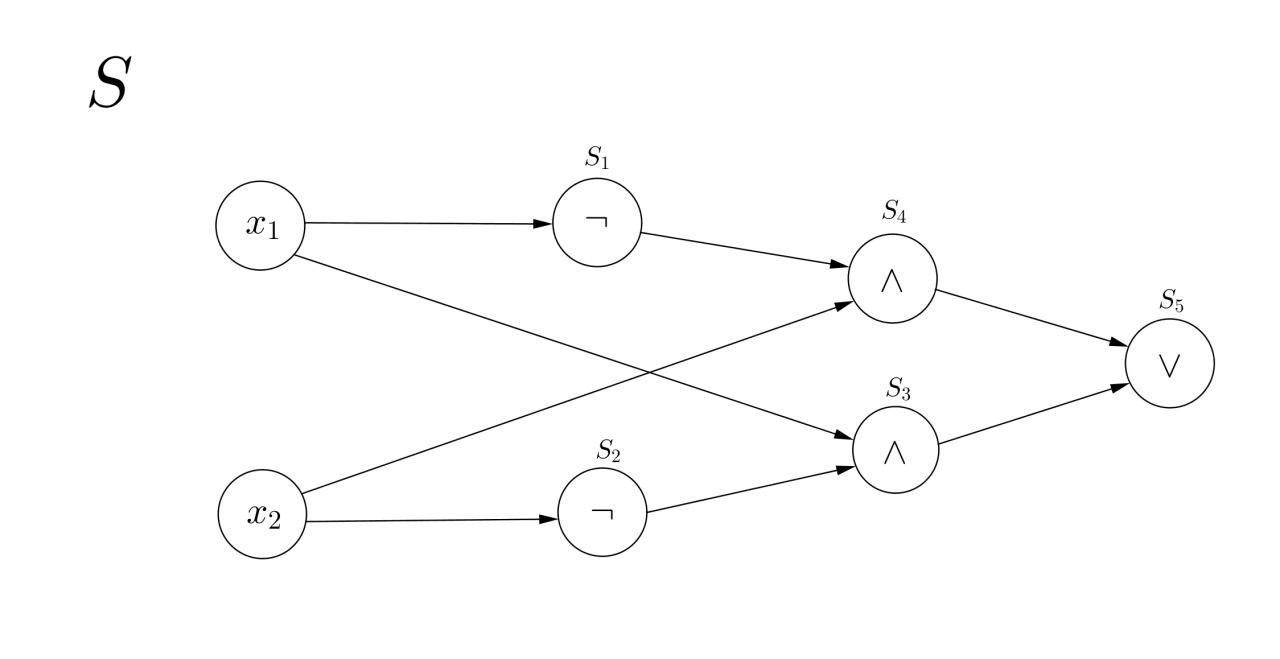
\includegraphics[height=7cm]{images/1.png}
 
 Если $x_2 = 0$, то $s_5 = x_1$
  
 Если $x_2 = 1$, то $s_5 = \lnot x_1$
 
 Результатом выполнения булевой схемы является сложение по модулю 2 (1, если значения $x_1$ и $x_2$ разные) - $\oplus$.
 
 \textsc{Пример 2}
 
 Составим схему, которая является сложением по модулю 2 $n$ переменных. Приведём индуктивное доказательство её существования: 
 
 \begin{enumerate}
     \item База индукции --- $n = 2$. Сложение 2 переменных по модулю 2 возможно по схеме, описанной выше
     \item Предположим существование такой схемы для $n - 1$ переменных 
     \[x_1 \oplus x_2 \oplus \ldots \oplus x_{n-1}\]
     \item Рассмотрим сложение по модулю 2 $n$ переменных. Представим его как сложение по модулю 2 $x_n$ с результатом предыдущего шага. Существование второго слагаемого объясняется предположением индукции. Сложение с $x_n$ можно выполнить по схеме выше. 
     \[x_1 \oplus x_2 \oplus \ldots \oplus x_{n-1} \oplus x_n = (x_1 \oplus x_2 \oplus \ldots \oplus x_{n-1}) \oplus x_n\]
 \end{enumerate}
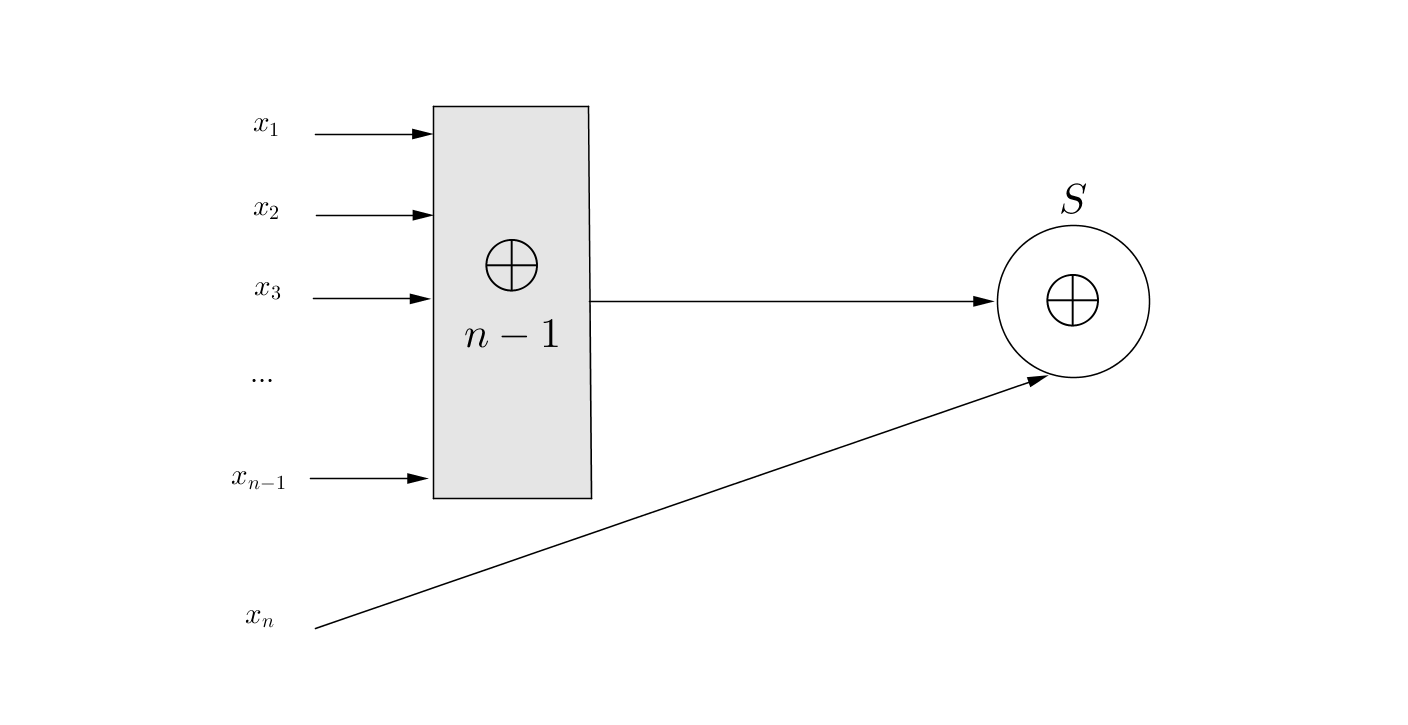
\includegraphics[height=7cm]{images/2.png}
 
 \textsc{Пример 3}
 
 Дизъюнкция n переменных --- аналогично, по индукции. Такие рассуждения можно построить и для конъюнкции.
 
 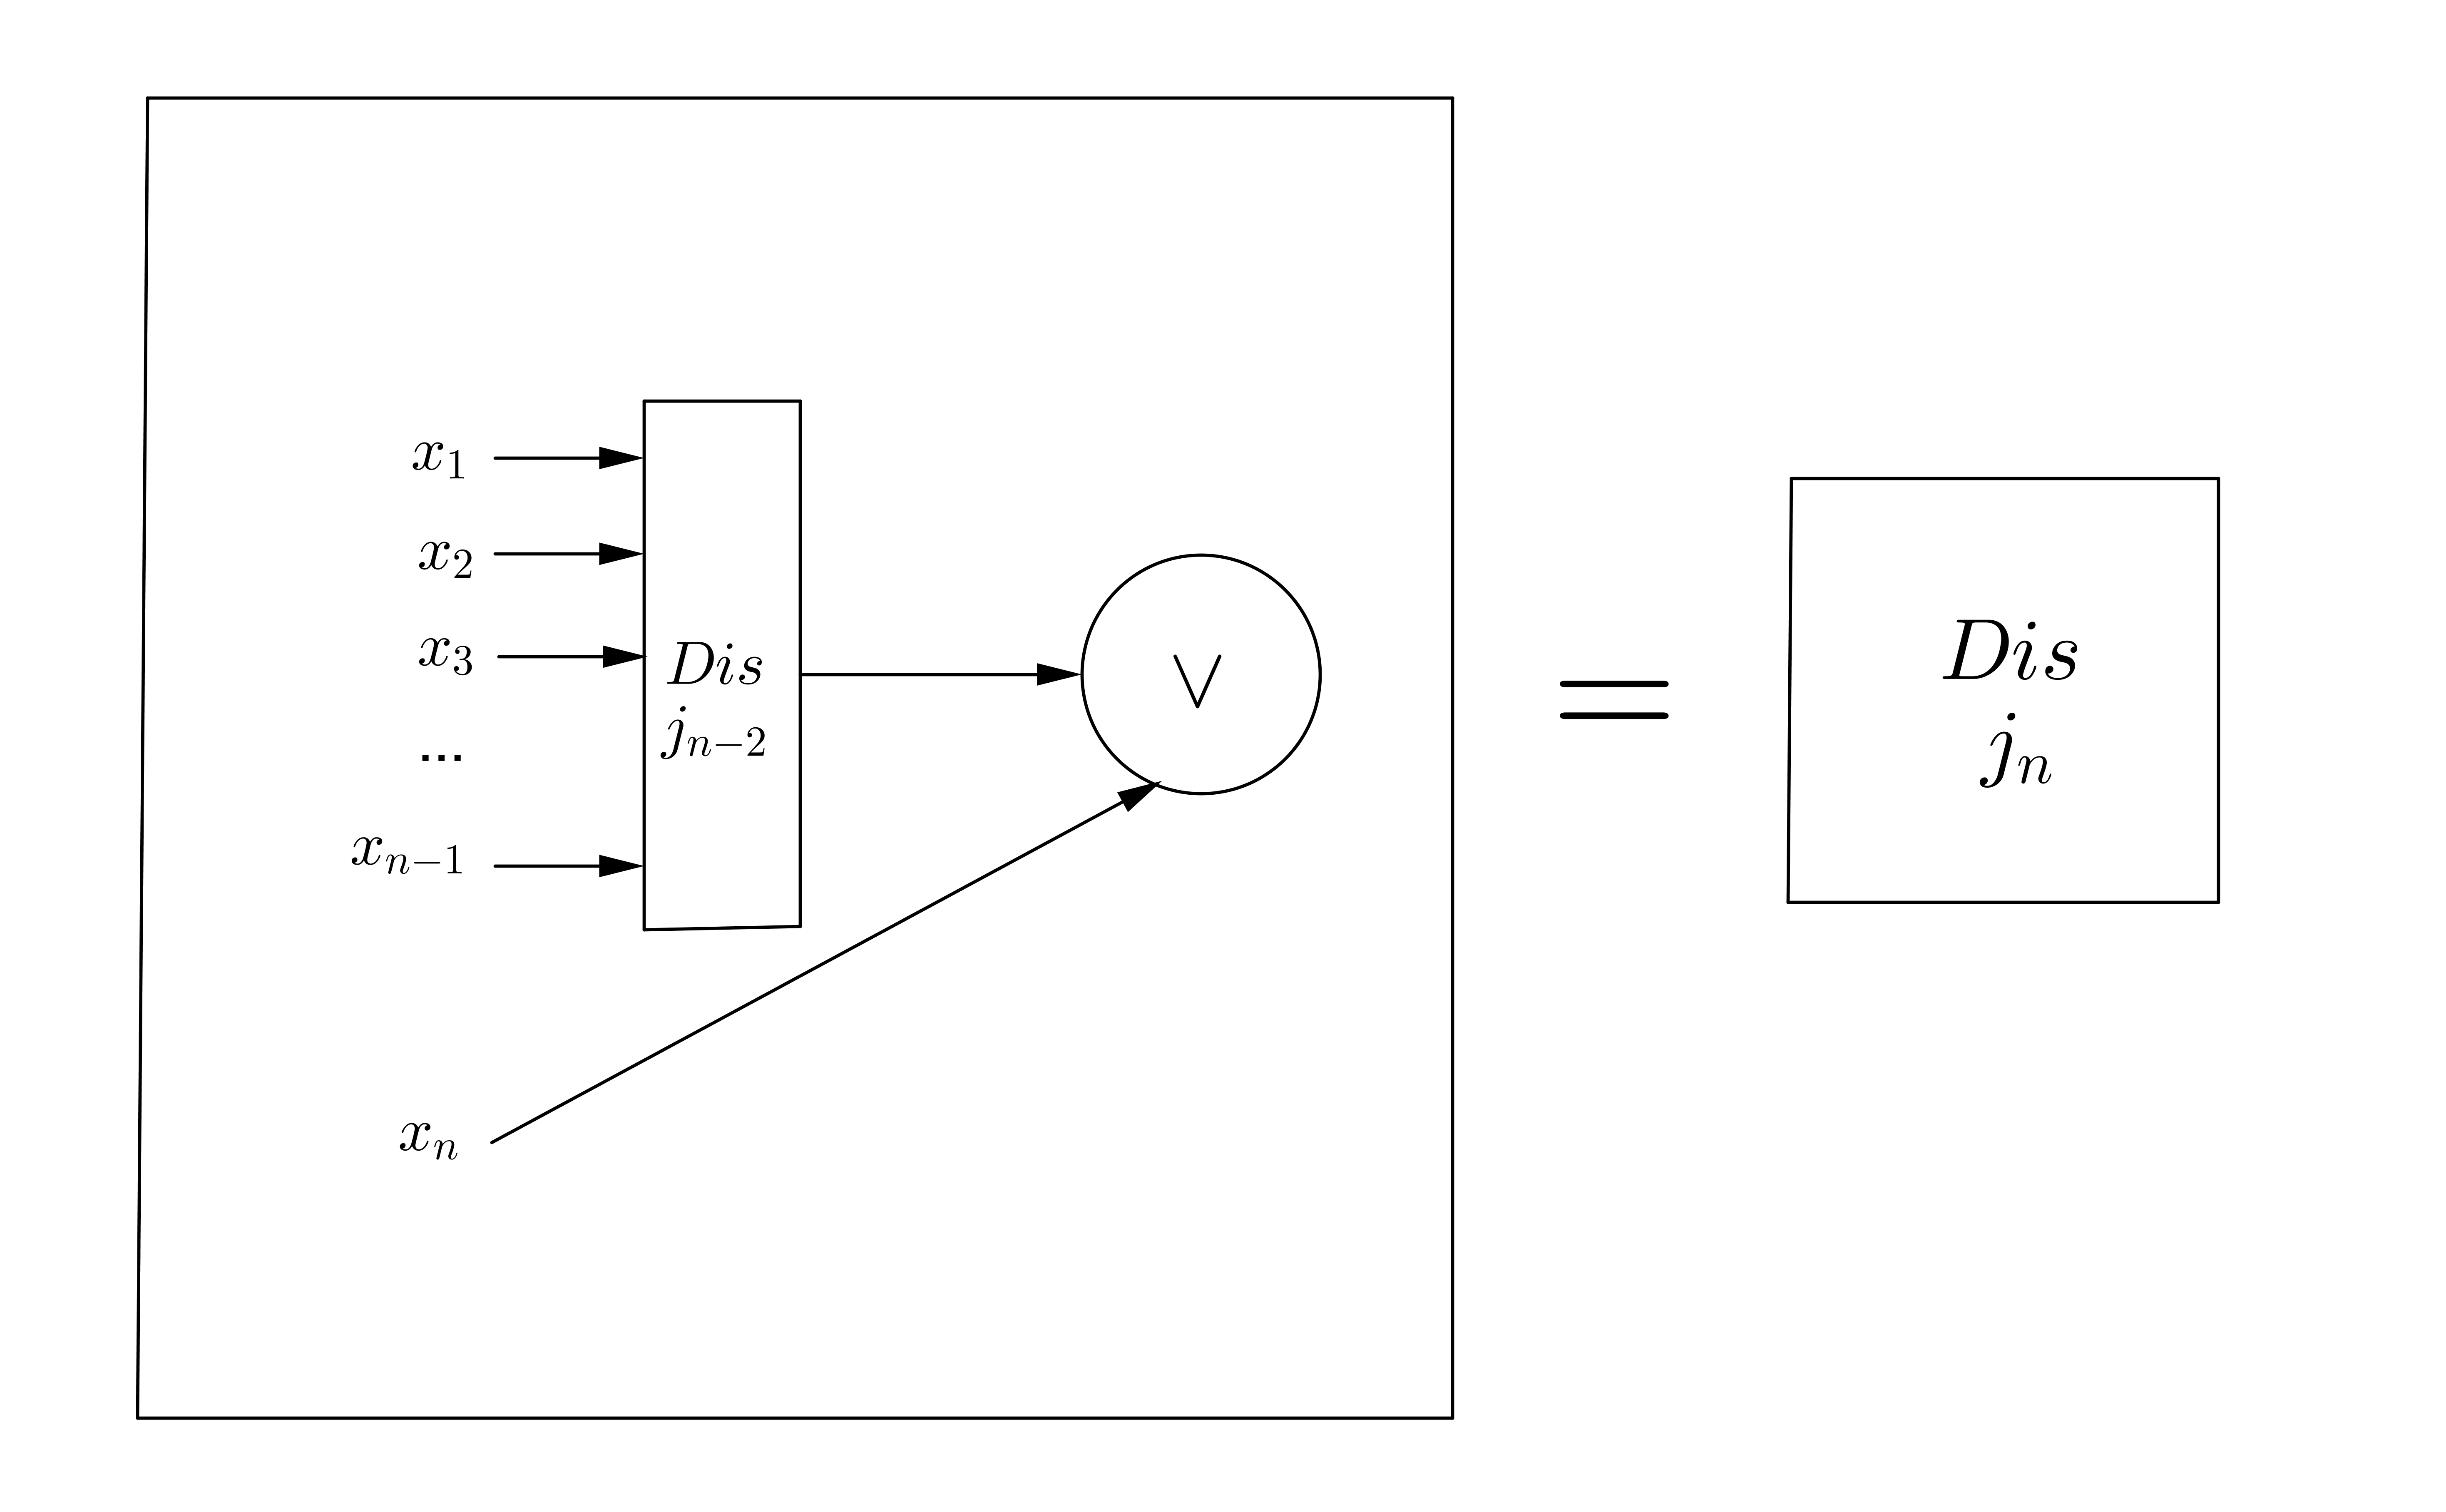
\includegraphics[height=7cm]{images/3.png}

\section*{11. Определение полного базиса. Примеры полных и неполных базисов.}

\textit{Полный базис: } Базис $B$ -- \textit{полный}, если любую булеву функцию можно вычислить схемой в базисе $B$.
 
Примеры полных базисов:

\begin{enumerate}
    \item Стандартный Базис
    \item Дизъюнкция, инверсия
    \item Конъюнкция, инверсия
    \item Импликация, инверсия
    \item Базис Жегалкина $\lbrace 	1, \oplus, \vee \rbrace$
    \item Стрелка Пирса
    \begin{enumerate}
        \item $0 \darr 0 = 1, 0 \darr 1 = 0, 1 \darr 0 = 0, 1 \darr 1 = 0$
        \item $X \darr X \equiv \neg X$  — отрицание
        \item $\left( {X \darr X} \right) \darr \left( {Y \darr Y } \right) \equiv {X  \wedge Y }$  — конъюнкция
        \item $\left( {X \darr Y} \right) \darr \left( {X \darr Y} \right) \equiv X \vee Y$  — дизъюнкция
        \item $\left( \left( {X \darr X } \right) \darr Y \right) \darr \left( \left( {X \darr X } \right) \darr Y \right) = X \rarr Y$  — импликация
    \end{enumerate}
    \item Штрих Шеффера
    \begin{enumerate}
        \item 0 \| 0 = 1, 0 | 1 = 1, 1 | 0 = 1, 1 | 1 = 0
        \item X\,|\,X  = \neg X  — отрицание
        \item \left( {X \,|\,X } \right)\,|\,\left( {Y \,|\,Y } \right) = X \vee Y  — дизъюнкция
        \item \left( {X \,|\,Y } \right)\,|\,\left( {X \,|\,Y } \right) = \left( {X  \wedge Y } \right)  — конъюнкция
        \item X \,|\, \neg X  — константа 1
    \end{enumerate}
\end{enumerate}

Примеры неполных базисов:

\begin{enumerate}
    \item Монотонный базис
    \item $\{\wedge,\oplus\}$
    \item $\{1,\wedge\}$
    \item $\{1,\oplus\}$
    \item Конъюнкция, дизъюнкция и разность
    \item Большинство одноэлементных базисов
\end{enumerate}

\section*{12. Определение схемной сложности функции.}

\textit{Размер булевой схемы} --- это количество присваиваний в схеме 
$g_1, \ldots, g_L$ для вычисления функции $f: \{0, 1\}^n \rightarrow \{0, 1\}$. 

\textit{Сложность функции f в базисе B} --- это минимальный размер булевой схемы, 
вычисляющей функцию $f$ в базисе B. Если базис не указывают -- имеют в виду 
стандартный базис $\{\lnot, \lor, \land\}$. \textit{Обозначение:} $C(f)$.

Определения различных оценок сложностей аналогичны тем, что мы используем на алгоритмах и в математическом анализе:

    \[
        o(f(n)) = \{g(n) \ | \ \forall \ c > 0 \ \exists \ n_0 > 0 \ : \forall n \geq n_0 \Rightarrow 0 \leq g(n) < c \cdot f(n)\}
    \]

    \[
        O(f(n)) = \{g(n) \ | \ \exists \ c > 0, \ \exists \ n_0 > 0 \ : \forall n \geq n_0 \Rightarrow 0 \leq g(n) \leq c \cdot f(n)\}
    \]

    \[
        \omega(f(n)) = \{g(n) \ | \ \forall \ c > 0 \ \exists \ n_0 > 0 \ : \forall n \geq n_0 \Rightarrow 0 \leq c \cdot f(n) < g(n)\}
    \]

    \[
        \Omega(f(n)) = \{g(n) \ | \ \exists \ c > 0, \ \exists \ n_0 > 0 \ : \forall n \geq n_0 \Rightarrow 0 \leq c \cdot f(n) \leq g(n)\}
    \]

    \[
        \Theta(f(n)) = \{g(n) \ | \ \exists \ c_1 > 0, \exists \ c_2 > 0, \exists \ n_0 \in \N: \ \forall \ n \geq n_0 \Rightarrow c_1 \cdot f(n) \leq g(n) \leq c_2 \cdot f(n)\}
    \]

\section*{13. Определение равномощных множеств. Основные свойства равномощности.}

\definition Равномощными множествами называются такие множества,
между которыми установима биекция. Обозначение: $A \sim B$.

\underline{Очевидные свойства равномощных множеств:} $\forall A$ -- множеств.
\begin{itemize}
        \item $A \sim A$.
        \item $A \sim B \Rightarrow B \sim A$.
        \item $A \sim B, B \sim C \Rightarrow A \sim C$.
\end{itemize}


\section*{14. Определение бесконечного множества.}

\definition Множество $A$ -- конечно тогда и только тогда,
когда $\exists n \in \N_0: A \sim [n]$ ($[n] = \left\{ 1, 2, \ldots, n \right\}, [0] = \varnothing$).

Запомните, что: $n > k \Rightarrow [n] \nsim [k]$.

\definition Множество бесконечно тогда и только тогда, когда оно не конечно.

\section*{15. Определение счетного множества. Примеры.}

$A$ -- бесконечно. Значит $A$ -- не пусто. $\exists a_o \in A$. 
Пусто ли $A\setminus {a_0}$? Нет. Иначе $A$ -- содержит один элемент и конечно.

Тогда $\exists a_1 \in A\setminus {a_0}$. Множество и без этих двух элементов 
бесконечно. Ну и так далее.

\definition Получившееся множество $A' = \{a_0, a_1, a_2, \ldots, a_n, \ldots\}$ 
назовем счётным (равномощным множеству натуральных чисел).
Биекция в этом случае очевидна: $f: i \mapsto a_i$.

\statement $\N$ -- бесконечно.
\begin{proof}
    Пусть это не так и $\exists f: [n] \to \N$ -- инъекция. Тогда верно следующее:
    $\N \ni max\{f(0), f(1), \ldots, f(n)\}+1 \notin f([n])$. А значит $f$ -- не биекция.
    А значит $\N$ не равномощно никакому $[n]$.
\end{proof}

\underline{Примеры cчётных множеств}:

\begin{itemize}
        \item $\{ 0, 1\}^*$ -- множество двоичных слов.
        \item $\N$ -- множество натуральных чисел (целые положительные и 0).
        \item $\N \times \N$ -- множество пар натуральных чисел.
        \item $\N^*$ -- множество конечных последовательностей натуральных чисел.
\end{itemize}

\statement Множество бесконечно тогда и только тогда, когда оно равномощно какому-то 
своему подмножеству.
\begin{proof}
    Докажем, что если множество бесконечно, то оно равномощно некоторому подмножеству.

    Как мы уже выяснили, в любом бесконечном множестве есть счётное подмножество.
    Пусть $B = \{b_0, b_1, \ldots, b_n, \ldots\}$ -- счётное подмножество
    бесконечного множества $A$.

    Установим биекцию $f: A \setminus \{b_0\} \to A$.
    \[
    f(x) = \begin{cases}
        b_{n-1}, x \in B \\
        x, x \notin B
    \end{cases}
    \]
    Получили то, что и требовалось.

    В обратную сторону доказывается на семинарах, но примерно так:
    пусть $B \subset A, B \sim A$. Пусть $A$ -- конечно. Тогда $|B| < |A|$
\end{proof}

\section*{16. Основные свойства счетных множеств.}

\begin{enumerate}
        \item
            \label{prop:AsubsetA}
            $A$ -- счётное множество. Тогда $A' \subseteq A$ счётно или конечно.
            \begin{proof}
                $A = \{a_0, a_1, \ldots, a_n, \ldots\}$. Вычеркнем все элементы, в $A'$
                не входящие. $A' = \{a_{j_0}, a_{j_1}, \ldots, a_{j_n}, \ldots\}$.

                Если последовательность $\{a_{j_n}\}$ конечна, то и $A'$ конечно.
                Если она бесконечна, то $A'$ очевидно счётно.
            \end{proof}
        \item 
            \label{prop:acupb}
            Если $A,B$ -- счётные, то и $A \cup B$ счётно.
            \begin{proof}
                $A = (a_0, a_1, \ldots, a_n, \ldots)$. 
                $B = (b_1, b_2, \ldots, b_n, \ldots)$.

                $A \cup B = (a_0, b_0, a_1, b_1 \ldots, a_n, b_n, \ldots)$.

                Но может получиться так, что в новой последовательности некоторые элементы
                встречаются по два раза (они входят в оба множества). Вычеркнем
                каждый такой элемент по одному разу. И получим последовательность,
                задающую счётное множество.
            \end{proof}
        \item $\Z$ -- счётно.
            \begin{proof}
                $Z = \N \cup (-\N)$ -- объединение счётных множеств. Счётно по свойству
                \ref{prop:acupb} ($-A = \{-a \ |\ a \in A\}$).
            \end{proof}
        \item 
            \label{prop:acupbnotinf}
            Если $A$ -- счётно, а $B$ -- конечно или счётно, то $A \cup B$ счётно.
            \begin{proof}
                Доказывается аналогично свойству \ref{prop:acupb}.
            \end{proof}
       \item Если $A$ -- счётно. И $B_1, B_2, \ldots, B_k$ -- счётны или конечны, то
            $A \cup B_1 \cup \ldots \cup B_k$ -- счётно.
            \begin{proof}
                К доказательству свойства \ref{prop:acupbnotinf} нужно добавить
                доказательство по индукции.
            \end{proof}
       \item
           \label{prop:Fsetcup}
           Счётное объединение конечных или счётных множеств конечно или счётно.

           $\{A_0, A_1, \ldots, A_n, \ldots\} = \mathfrak{F} \sim \N$. $A_i$ -- множество.
           $\mathfrak{F}$ называется семейством множеств. 
           $A = \bigcup\limits_{i=0}^{\infty} A_i$.

           \statement $A$ -- счётно.
           \begin{proof}
               \begin{align*}
                   A_0 &= (a_{00}, a_{01}, \ldots, a_{0n}, \ldots) \\
                   A_1 &= (a_{10}, a_{11}, \ldots, a_{1n}, \ldots) \\
               \end{align*}
               Некоторые из множеств могут быть конечны. Дополним их до счётных
               пустым символом $\lambda \notin A$.

               Построим последовательность: $a_{00}, a_{01}, a_{10}, a_{02},
               a_{11}, a_{20}, \ldots$. (то есть проходим последовательно все значения
               сумм индексов от $0$ до $\infty$).

               Теперь исключим из последовательности повторения и символы $\lambda$.
               Получим требуемую последовательность $(a'_0, a'_1, \ldots, a'_n, \ldots)$.

               Теперь получим функцию $f: [n] \to A$ или $f: \N \to A$. $f$ -- биекция.
               В первом случае множество конечно, во втором счётно.

               Можно было бы и не вводить $\lambda$, а исключать эти элементы сразу,
               но так проще (нет никаких условий).
           \end{proof}

           \underline{Примеры:} 
           \begin{itemize}
                \item Пусть $A_i = \{i\}$. Тогда $A = \N$ (счётно).
                \item Пусть $A_i = \{1\}$. Тогда $A = \{1\}$ (конечно).
           \end{itemize}

      \item
          \label{prop:CartProdAB}
          Декартово произведение счётных множеств счётно.
          Напомним, что \[A \times B = \left\{ (a; b)\ |\ a \in A, b \in B \right\}\]
          \begin{proof}
              По определению декартово произведение есть множество всех упорядоченных пар вида $\langle a,\ b\rangle$, в которых $a \in A$ и $b \in B$. Разделим пары на группы, объединив пары с одинаковой первой компонентой (каждая группа имеетвид $\{a\} \times B$ для какого-то $a \in A$). Тогда каждая группа счётна, поскольку находится во взаимно однозначном соответствии с $B$ (пара определяется своим вторым элементом), и групп столько же, сколько элементов в $A$, то есть счётное число.
          \end{proof}
      \item 
          \label{prop:Apown}
          Если $A$ -- счётно, то $A^k$ -- счётно.
          \begin{proof}
              Очевидно по индукции из свойства \ref{prop:CartProdAB}.
          \end{proof}
      \item $\Q$ -- счётно.
          \begin{proof}
              Рассмотрим множество $\Q_p$ несократимых дробей. 
              Пусть функция $f: \Q_p \to \Z \times \N_+$ -- инъекция
              (она переводит дробь в пару чисел числитель-знаменатель).
              Тогда она является биекцией на $f(\Q_p) \subset \Z \times \N_+$. 
              Причём $f(\Q_p)$ тогда счётно по свойству \ref{prop:AsubsetA}
              так как не является конечным, а $\Z \times \N_+$ счётно
              по свойству \ref{prop:CartProdAB}.
          \end{proof}
      \item Пусть $A^*$ -- конечные последовательности конечного (непустого) или 
          счётного алфафита $A$.

          \statement $A^*$ -- счётно
          \begin{proof}
              $A^* = \bigcup\limits_{n=0}^{\infty} A^n$. При этом $A^n$ -- слова длины $n$.
              $A^n$ -- счётно по свойству \ref{prop:Apown}. И тогда само $A^*$ счётно
              по свойству \ref{prop:Fsetcup}.
          \end{proof}
      \item \definition $\alpha \in \R$ -- алгебраическое число тогда и только тогда, 
          когда $\alpha$ -- корень некоторого многочлена с целыми коэфициентами.

          \statement Множество алгебраических чисел счётно.
          \begin{proof}
              Приведём только план доказательства:
              \begin{enumerate}
                      \item Докажем, что многочленов степени $n$ ($n \in \N$) с целыми коэфициентами счётно.
                      \item Для каждого из этих многочленов есть не более $n$ корней --
                          алгебраических чисел.
                      \item Удаляем повторяющиеся корни.
                      \item Получим все алгебраические числа, которых, очевидно, 
                          счётно.
              \end{enumerate}
          \end{proof}
\end{enumerate}

\section*{17. Определение множества мощности континуум. Примеры.}

Определим действительные числа следующим образом: сопоставим каждому $x \in \R$ двоичное число: $\pm \lefteqn{\underbrace{\phantom{10110 \dots 1011}}_{\text{целая часть}}}10110 \dots 1011 .\overbrace{110001 \dots 00110}^{\text{дробная часть}}$. Считаем известным, что ряд из каких-то степеней двоек сходится, причём запрещаем в числах данного вида "хвосты из единиц".

\definition Будем говорить, что множество $X$ имеет мощность континуум, если $X \sim \R$.

Примеры:

\begin{itemize}
        \item $\Phi(\N)$ -- множество всех подмножеств $\N$.
        \item $2^{\N}$ -- множество последовательностей натуральных чисел.
        \item $\R$ -- само множество действительных чисел.
\end{itemize}

\section*{18.  Основные свойства континуальных множеств.}

\begin{enumerate}
    \item Любое континуальное множество имеет счётное подмножество.
    \item Мощность объединения не более чем континуального количества множеств, каждое из которых не более чем континуально, не превосходит континуума.
    \item При разбиении континуального множества на конечное или счётное число частей хотя бы одна из частей будет иметь мощность континуум.
\end{enumerate}

\section*{19.  Основные свойства вычислимых функций.}

\definition{Функция называется вычислимой, если для неё существует некоторый алгоритм вычисления.}

\begin{algo1}
Композиция вычислимых функций вычислима.
\end{algo1}
\begin{proof}
Пусть существуют вычислимые функции $f$, переводящая множество входов $X$ в множество выходов $Y$ и $g$, переводящая $Y$ в $Z$.

\[
    \begin{cases}
        f: X \to Y \\
        g: Y \to Z
    \end{cases}
\]

Построить $g \circ f: X \to Z$ достаточно просто. На первом шаге нужно применить функцию $f$. Далее берём множество выходов $f$ и подаём на вход в $g$. На выходе получим некоторое множество выходов $Z$. Вычислимая композиция построена.

\begin{algorithm}
\caption{Алгоритм получения композиции функций}
\begin{algorithmic}[1]
\Function{Composition}{x}
    \State $t \gets f(x)$
    \State \Return $g(t)$
\EndFunction
\end{algorithmic}
\end{algorithm}
\end{proof}

Итак, есть вычислимая биекция $\pi: \N^* \to \N$.

Построим композицию $\N^* \to \N \to \{0, 1\}$.

\[
    \begin{cases}
        \pi^{-1}: B \to A \\
        f: A \to A \\
        \pi: A \to B
    \end{cases}
\]

Построить это можно применением композиции  $\pi \circ f \circ \pi^{-1}$. Получим алгоритм из $B$ в $B$. 
Поэтому нам, по сути, \textbf{без разницы какие множества на входе
и выходе} так как можно получить легко из одного другое.

Заметим, что если некоторая биекция $\pi$ вычислима, то обратная ей $\pi^{-1}$ также будет вычислима. Способ вычисления схож с алгоритмом для диофантовых уравнений.

Рассматриваем все возможные значения входов и вычисляем $\pi^{-1}(x)$.
\begin{algorithm}
\caption{Алгоритм построения обратной функции для биекции}
\begin{algorithmic}[1]
\Function{RevBiection}{x}
    \For{$n := 0 \ldots \infty$}
        \If{$\pi(n) = x$} 
            \State \Return n
        \EndIf
    \EndFor
\EndFunction
\end{algorithmic}
\end{algorithm}

Стоит отметить, что данный алгоритм всегда завершается так как
(по определению) биекция сюрьективна и найдется номер $n$ для
которого $\pi(n) = x$.

\section*{20. Определение разрешимого множества.}

Вспомним что такое характеристическая функция множества $S$:
\[
\chi_S(x) = \begin{cases}
    1,\ x \in S \\
    0,\ x \notin S
\end{cases}
\]

\definition{Множество называется разрешимым, если его
характеристическая функция вычислима.}

\section*{21. Определение перечислимого множества.}

\definition{Алгоритм перечисления -- такой алгоритм, у которого нет входа, он работает и может выводить некоторые числа, причём все напечатанные числа составляют счетное множество.}

\definitionone{Множество $S$ называется перечислимым, если есть алгоритм перечисления всех его элементов.}

\definitiontwo{Множество $S$ -- перечислимо, если существует такая вычислимая функция:

\[
    f: \N \to \N
    \begin{cases}
        f(\N) = S \\
        \text{Область определения} \ f \ \text{равна либо} \ \N, \text{либо} \ [n].
    \end{cases}
\]

}

\begin{theorem}

Определения $1$ и $2$ эквивалентны.

\end{theorem}

\begin{proof}
\ 

$\Longrightarrow$
Пусть $A$ -- алгоритм перечисления множества $S$. Тогда возьмём следующий алгоритм $B$: принимает на вход число $n$, запускает алгоритм $A$ и считает, сколько чисел напечатано. Как только вывели $n + 1$ слово -- алгоритм печатает результат.

Покажем, что соблюдаются свойства вычислимой функции:

\begin{enumerate}
    \item $B(n) = S$, так как $\forall \ n \ \exists \ B(n) \Rightarrow 
    \begin{cases}
        \forall \ x \in S \ \exists \ B(x) \\
        \forall \ x \notin S$ никогда не выведет $B(x)
        \end{cases}$
    \item Пусть $S$ -- бесконечное множество, тогда функция, задаваемая $B$, определена везде, значит $dom \ B = \N$. Если $B$ работает на $n$ числах, то алгоритм переберёт их и остановится.
\end{enumerate}

$\Longleftarrow$
Возьмём следующий алгоритм перечисления $B$ для множества $S$:

\begin{algorithm}
\caption{Алгоритм перечисления разрешимого множества}
\begin{algorithmic}[1]
\Function{PrintSet}{S}
    \For{$i := 0 \ldots \infty$}
        \If{$f(i) = 1$} 
            \State \textbf{print} i
        \EndIf
    \EndFor
\EndFunction
\end{algorithmic}
\end{algorithm}

Если функция определена для некоторых $n$ чисел, то ровно их он и напечатает. Если $dom \ f = \N$, то алгоритм никогда не остановится, то есть напечатает всю область определения $f$. Значит, существует алгоритм, перечисляющий $S$.

\end{proof}

\section*{22. Свойства перечислимых множеств.}

\statement{
Если множество $S$ разрешимо, то оно перечислимо.
}

\begin{proof}
Алгоритм перечисления множества $S$ использует алгоритм раз-
решения множества $S$. Он перебирает все числа, начиная с 0; для каждого числа
$n$ вычисляет индикаторную функцию $\chi S(n)$ и печатает число n, если полученное
значение равно 1.

            \begin{algorithm}
            \caption{Алгоритм перечисления множества S}
            \begin{algorithmic}[1]
            \Function{Print}{S(n)}
                \For{$n := 0 \ldots \infty$}
                    \If{$\chi_{S}(n) = 1$}
                        \State \textbf{print} n
                    \EndIf
                \EndFor
            \EndFunction
            \end{algorithmic}
            \end{algorithm}
            
Корректность такого алгоритма ясна из определений.
\end{proof}

Пусть $S$ -- перечислимое непустое множество. Тогда для $S$ выполнены следующие свойства:

\begin{enumerate}
        \item $S$ -- область определения вычислимой функции.
        \item $S$ -- область значений вычислимой функции.
        \item $S$ -- область значений всюду определённой вычислимой функции.
\end{enumerate}
    
Пусть $A$ и $B$ -- перечислимые множества. Тогда:

\begin{enumerate}
    \item $A \cup B$ перечислимо.
    \item $A \cap B$ перечислимо.
\end{enumerate}

\statement{
    Существует перечислимое неразрешимое множество.
}

\begin{proof}
    Рассмотрим вычислимую функцию $f(x)$, не имеющую всюду определённого вычислимого продолжения. Её область определения $F$ будет искомым множеством. В самом деле, $F$ перечислимо (по одному из определений перечислимости). Если бы $F$ было разрешимо, то функция
    
    \[
        g(x) =
        \begin{cases}
            f(x), \text{если $x \in F$} \\
            0, \text{если  $x \notin F$}.
        \end{cases}
    \]
    
    была бы вычислимым всюду определённым продолжением функции $f$ (при вычислении $g(x)$ мы сначала проверяем, лежит ли $x$ в $F$, если лежит, то вычисляем $f(x)$).
\end{proof}

\section*{23. Определение универсальной вычислимой функции.}

\definition{Универсальная вычислимая функция:

    \[
        U : \N \times \N \to \N\ | \ \forall f\text{-вычислимая}\ \exists \ p: f(x) = U(p,\ x).
    \]

}

Также полезно знать про отладочную функцию:

\definition{Отладочная функция:

    \[
        F: \N\times\N\times\N \to \{0,\ 1\}\text{ -- всюду определённая, причём: }
    \]
    
    \[
        \begin{cases}
            \text{При фиксированных $p$ и $x$ монотонна по $t$}\\
            F(p,\ x,\ t) = 0 \Leftrightarrow U(p,\ x)\text{ не определена}\\
            F(p,\ x,\ t) = 1 \Leftrightarrow \text{ программа $p$ на входе $x$ заканчивает работу за $t$ шагов.}
        \end{cases}
    \]
}

\section*{24. Определение главной универсальной вычислимой функции.}

\definition{Главная универсальная функция (гёделева) -- такая универсальная функция, 
что для любой вычислимой функции $V(n,\ x)$ существует всюду определённая
вычислимая функция $s(n)$, что:
    \[
        \forall\ n,\ x \Rightarrow V(n,\ x) = U(s(n),\ x).
    \]
}

Неформально это значит, что главная универсальная функция позволяет транслировать
в себя любую другую унивесальная функция. Ну, вот например, есть язык C++, его можно
назвать главной универсальной функцией так как любую программу на другом универсальном
языке можно переписать на C++ автоматически (при помощи \emph{транслятора}).

\section*{25. Формулировка теоремы Успенского–Райса.}

Пусть есть некоторое свойство, которое мы хотим проверить
для некоторой функции. 

Формально:
Пусть $\{f:\N\to\N\}$ -- множество вычислимых функций. 
Разделим его на два непересеающихся подмножества $A$ и $\overline{A}$.
\[
\{f\ |\ f:\N\to\N\} = A \cup \overline{A}
\]
$A$ -- множество тех функций, для которых выполняется некое свойство,
$\overline{A}$ -- множество тех функций, для которых это свойство не выполняется.

Возьмём некоторую универсальню функцию $U(p,\ x)$.

Обозначим за $P_A$ множество всех $p$ таких, что $U(p,\ x) \in A$.
\[
P_A = \{p\ |\ U(p, x) \in A\}
\]

Тогда вопрос можно поставить так: разрешимо ли множество
программ, удовлетворяющих нашему свойству? На этот вопрос и отвечает теорема
Успенского-Райса:
\begin{usp-rais}
   Если $A$ -- нетривиально ($A \neq \oslash,\ \overline{A} \neq \oslash$), а $U(q,\ x)$ -- главная универсальная функция, то множество $P_A$ неразрешимо.
\end{usp-rais}
Введём для удобства ещё функции $\varepsilon \in \overline{A}$ (нигде не 
определённая) и $\xi \in A$ (какая-то функция, удовлетворяющая условию).
Сделать это можно по аксиоме выбора.

Если $A$ -- это множество нигде не определённых функций, то поменяем их
местами так как $P_A$ разрешимо тогда и только тогда, когда его
дополнение разрешимо.

\section*{26. Формулировка теоремы о неподвижной точке.}

\begin{point}
    Пусть $U$ -- главная универсальная функция, $h(n)$ -- любая всюду определённая вычислимая функция. Тогда:
    
    \[
        \exists\ q \ : \ U(q,\ x) = U(h(q),\ x).
    \]
\end{point}

Честно сказать, не все учёные понимают эту теорему, однако её можно объяснить неформально
так: для любой программы на любом универсальном языке существует ещё одна программа,
которая делает то же самое (то есть программы совпадают).

\section*{27.1. Определение машины Тьюринга (с одной лентой).}

Мы рассмотрим классическую модель вычислений, на которой будут основано точное определение вычислимых функций, -- машины Тьюринга (МТ).

МТ состоит из

\begin{itemize}
    \item бесконечной в две стороны ленты, в ячейках которой могут быть записаны символы алфавита $A$ (некоторого конечного множества)
    \item головки, которая может двигаться вдоль ленты, обозревая в каждый данный момент времени одну из ячеек
    \item оперативной памяти, которая имеет конечный размер (другими словами, состояние оперативной памяти -- это элемент некоторого конечного множества, которое называется множеством состояний МТ $Q$)
    \item таблицы переходов (или программы), которая задаёт функцию $\delta : A \times Q \to A \times Q \times \{-1,\ 0,\ +1\}$
\end{itemize}

Поскольку таблица переходов -- это функция на конечном множестве, её возможно задать таблицей. Каждая строка таблицы -- это пять значений $a,\ q,\ a^{'},\ q^{'},\ d$, (другие способы записи: $\delta(a,\ q) = (a^{'},\ q^{'},\ d)$ или $\delta : (a,\ q) \mapsto (a^{'},\ q^{'},\ d))$, которые описывают следующий порядок действий МТ: если головка МТ находится над ячейкой, содержащей символ $a$, а состояние МТ равно $q$, то на очередном такте
работы МТ записывает в текущую ячейку символ $a^{'}$, изменяет состояние на $q^{'}$ и сдвигает головку на $d$ ячеек (отрицательное значение отвечает сдвигу влево, положительное -- сдвигу вправо, $0$ -- не сдвигается).

Работа МТ состоит из последовательного выполнения тактов в соответствии с таблицей переходов. Может так случиться, что для текущей пары значений $(a,\ q)$ функция переходов не определена. В этом случае работа машины заканчивается (машина останавливается). Обычно среди состояний МТ выделяют множество $Q_f$ финальных состояний -- таких состояний $q_f$, что таблица переходов не определена для всех пар $(a,\ q_f)$. Попав в финальное состояние, машина обязательно остановится, отсюда и название. 

Лента МТ бесконечна и это не соответствует нашей интуиции об алгоритмах: алгоритм на каждом шаге работы оперирует лишь данными конечного размера. Чтобы учесть это обстоятельство, мы предполагаем, что в алфавите машины есть специальный символ $\Lambda$ (пробел или пустой символ) и все ячейки ленты за исключением конечного числа содержат пустые символы. Это свойство ленты сохраняется при работе МТ, поскольку за такт работы меняется содержимое не более одной ячейки ленты.

Состояние такой машины уже описывается конечными данными. Мы будем использовать конфигурации. Конфигурация -- это слово в алфавите $A \cup Q$, в котором первый и последний символы непустые, и ровно один символ принадлежит множеству состояний. Договоримся считать, что символ состояния записывается слева от символа в той ячейке, над которой находится головка МТ. На ленте слева и справа от символов конфигурации стоят только пустые
символы.

У МТ есть 2 основных конфигурации: начальная $q_0$, из которой МТ начинает работу, и финальная $q_f$.

Конфигурации МТ преобразуются такт за тактом, порождая последовательность конфигураций $c_0 = q_0u,\ c_1,\ c_2, \ldots ,\ c_t,\ \ldots$

Эта последовательность бесконечна, если машина не останавливается, и конечна в
противном случае. Результатом работы является та часть финальной конфигурации, которая расположена между символом состояния и ближайшим к нему пустым символом справа.

\section*{27.2. Определение машины Тьюринга (с несколькими лентами).}

\definition{Машина, у которой не одна лента, а несколько
(фиксированное число для конкретной машины), называется \textit{многоленточной}.}

На каждой ленте есть своя головка. За такт работы головки могут перемещаться по всем лентам. Действие на такте работы зависит как от состояния машины, так и от всего набора символов, которые
видят головки машины на всех лентах.

Чтобы задать машину с $h$ лентами, нужно указать: 

\begin{itemize}
    \item алфавит $A$, в котором выделен пустой символ $\Lambda$
    \item множество состояний $Q$, в котором выделено начальное состояние $q_0$
    \item таблицу переходов, которая теперь является функцией вида $\delta : A^h \times Q \to A^h \times Q \times \{-1, 0, +1\}^h$ (первый аргумент -- символы, которые машина видит на ленте, последний -- команды движения для головок на каждой ленте).
    \item выделить среди лент ленту входа и ленту результата (возможно, что это одна и та же лента)
\end{itemize}

Таблица переходов по прежнему является функцией на конечном множестве, поэтому её возможно задать таблицей.
Работа МТ состоит из последовательного выполнения тактов в соответствии с таблицей переходов. Может так случиться, что для текущего набора значений $(a_1, a_2, \ldots ,\ a_h,\ q)$ функция переходов не определена. В этом случае работа машины заканчивается (машина останавливается). Как и раньше, можно ввести множество финальных состояний $Q_f$, т.е. тех состояний $q_f$, для которых таблица переходов не определена для всех значений $(a_1, a_2, \ldots ,\ a_h,\ q_f)$. В финальном состоянии машина обязательно останавливается.

Мы предполагаем, что $h$-МТ начинает работу в состоянии $q_0$, а все ленты кроме ленты входа содержат только пустые символы. На ленте входа записано входное слово, и головка находится над первой слева ячейкой, содержащей символы этого
слова. Поскольку за такт работы меняется содержимое не более одной ячейки ленты, в процессе работы машины на каждой ленте будет записано лишь конечное количество непустых символов.

Конфигурация многоленточной машины может быть задана набором конфигураций на каждой ленте $(u_1q_{v_1},\ u_2q_{v_2}, \ldots ,\ u_hq_{v_h})$.

Символ состояния один и тот же, так как по нашим определениям состояние есть у машины, а не у головки.

Далее нам будет удобен другой способ представления конфигурации машины. Выровняем ленты и будем рассматривать \textit{окно}, в которое заведомо помещаются все непустые символы на каждой ленте. В таком случае конфигурация однозначно определяется матрицей размера $h \times N$, в которой записаны символы на лентах. Нужно ещё указать положения головок на лентах (они-то не обязательно выровнены -- машина способна перемещать головки независимо). По этой причине будем помещать в матрицу не символы алфавита $A$, а пары $(a, \hat{q})$, где $\hat{q}$ указывает, расположена ли на данной ленте головка над данной ячейкой. Если да, то $\hat{q} \in Q$ -- текущее состояние машины. Если нет, то $\hat{q}$ -- какой-то символ не из $Q$, который указывает,
что над над данной ячейкой на данной ленте нет головки. Будем для единообразия использовать в качестве такого символа $\Lambda$. Такую матрицу в дальнейшем называем
матрицей конфигурации. Вот пример матрицы начальной конфигурации для двухленточной машины:

\begin{figure}[h]
\begin{center}
    \begin{minipage}[h]{0.6\linewidth}
        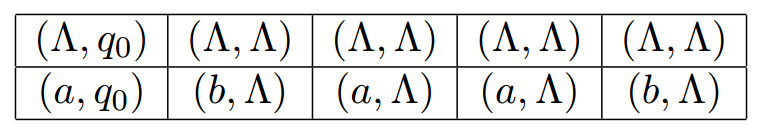
\includegraphics[height=1.75cm, width=\linewidth]{images/TabMT.png}
    \end{minipage}
\end{center}
\end{figure}

Как и для одноленточной машины, работа $h$-МТ порождает последовательность конфигураций $c_0 = q_0u,\ c_1,\ c_2, \ldots ,\ c_t,\ \ldots$

Эта последовательность бесконечна, если машина не останавливается, и конечна в противном случае. Результатом работы является та часть финальной конфигурации на ленте результата, которая расположена между положением головки и ближайшим к нему пустым символом справа. Например, если у двухленточной МТ
лента результата -- нижняя, то результатом работы МТ, остановившейся в конфигурации, заданной окном

\begin{figure}[h]
\begin{center}
    \begin{minipage}[h]{0.6\linewidth}
        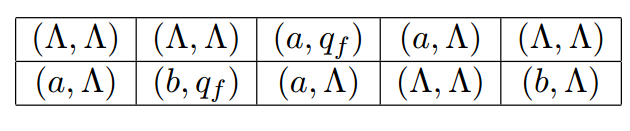
\includegraphics[height=2cm, width=\linewidth]{images/Tab2MT.png}
    \end{minipage}
\end{center}
\end{figure}

будет $ba$.

\section*{28.  Определение функции, вычислимой на машине Тьюринга.}

\definition{МТ $M$ ($h$-МТ, если многоленточная) вычисляет функцию $f : B^{*} \to B^{*}$ (где $B$ -- подмножество алфавита машины, не содержащее пустого символа), если для каждого $w$ из области определения функции $f$ результат работы $M$ равен $f(w)$, а для каждого $w$ не из области определения $f$ машина $M$ не останавливается на входе $w$. 
}

Функция $f$ называется \textit{вычислимой машинами Тьюринга}, если есть такая МТ, которая вычисляет $f$.


\end{document}
